\chapter{Física nuclear}\label{ch:b3:nuclear-physics}

% Provenance (not for print): first half of the "physique subatomique"
% module common to the surveyed third-year curricula; particle physics
% follows in the next chapter. Deepens the high-school volume's
% radioactivity with SEMF, Gamow tunnelling and reactor physics.

O volume do ensino médio contou o esboço da história: os átomos têm
núcleos; alguns núcleos se desfazem, em prazos que vão de microssegundos
a bilhões de anos; e gramas de matéria escondem megatons de energia. Este
capítulo reabre o núcleo com as ferramentas do terceiro ano. Um modelo de
gota com cinco termos prevê a ligação de centenas de \omterm{def:b3:nuclear-physics:nuclide}{nuclídeos} com
precisão de por cento; o tunelamento quântico --- o problema da barreira
do volume do segundo ano, promovido --- explica como uma só fórmula cobre
vinte e cinco ordens de grandeza nos tempos de vida do decaimento
$\alpha$; e o discreto máximo da curva de \omterm{prop:b3:nuclear-physics:binding}{energia de ligação} no ferro
divide toda a tecnologia nuclear em dois campos: partir os pesados
(reatores) ou juntar os leves (as estrelas e, um dia, as usinas). O
capítulo termina à beira de uma piscina de reator, brilhando no azul de
Cherenkov.

\section{O núcleo: uma gota saturada}

\begin{definition}[Nuclídeos, tamanho e densidade]\label{def:b3:nuclear-physics:nuclide}
\index{nuclídeo}\index{isótopo}\index{raio nuclear}
Um \emph{nuclídeo} $^{A}_{Z}\text{X}$ guarda $Z$ prótons e $N = A -
Z$ nêutrons, ligados pela \emph{interação forte}: intensa
(${\sim}\qty{100}{}\times$ a de Coulomb no contato), de curto alcance
(${\sim}\qty{1}{fm}$, sentida só pelos vizinhos que se tocam) e cega
à carga (ela agarra prótons e nêutrons por igual). Os experimentos de
espalhamento dão a todo núcleo a mesma receita: raio
\[
R = r_0A^{1/3} , \qquad r_0 \approx \qty{1.2}{fm} ,
\]
e assim o volume cresce como $A$ e a densidade é um valor universal,
$\rho \approx \qty{2.3e17}{kg/m^3}$ --- uma gota de chuva disso pesaria
como uma frota de petroleiros, e o
\cref{ch:b3:astrophysics} encontrará estrelas inteiras nesta densidade.
Os \emph{isótopos} compartilham o $Z$, mas diferem no $N$: mesma química,
destinos nucleares diferentes.
\end{definition}

\begin{proposition}[Defeito de massa e energia de ligação]\label{prop:b3:nuclear-physics:binding}
\index{defeito de massa}\index{energia de ligação}\index{pico do ferro}
Um núcleo ligado pesa \emph{menos} que as partes dele; pelo
\cref{ch:b3:relativistic-dynamics}, a massa que falta é a
\omterm{prop:b3:nuclear-physics:binding}{energia de ligação},
\[
B = \big(Zm_{\text{p}} + Nm_{\text{n}} - m_{\text{núcleo}}\big)c^2 ,
\]
tipicamente ${\sim}\qty{8}{MeV}$ \emph{por núcleon} --- um milhão
de vezes a química. Traçado por núcleon, o $B/A$ sobe abruptamente pelos núcleos leves
(os efeitos de superfície somem), tem máximo em $\approx\qty{8.8}{MeV}$ perto do
ferro-56 e então declina à medida que a repulsão de Coulomb, de longo
alcance e sem saturação, taxa os pesos-pesados. As duas encostas são
minas de energia: a \emph{fusão} sobe a da esquerda (o negócio do Sol) e
a \emph{fissão} desce a da direita (o do reator) --- e o ferro,
no cume, é cinza nuclear para as duas.
\end{proposition}

\begin{omfigure}
\begin{tikzpicture}
  \begin{axis}[omaxis, axis x line=bottom, axis y line=left,
    width=11.2cm, height=6.2cm, xmin=0, xmax=250, ymin=0, ymax=10.3,
    xlabel={número de massa $A$}, ylabel={$B/A$ (\unit{MeV})},
    xlabel style={at={(axis description cs:0.5,-0.1)}, anchor=north},
    xtick={56,100,150,200,238}, ytick={2,4,6,8}, clip=false]
    \addplot[omDef, very thick, smooth] coordinates {
      (2,1.11) (3,2.7) (6,5.3) (9,6.46) (12,7.68) (16,7.98)
      (24,8.26) (40,8.55) (56,8.79) (75,8.7) (100,8.6)
      (125,8.45) (150,8.3) (175,8.1) (200,7.9) (220,7.75) (238,7.57)};
    \fill[omThm] (axis cs:4,7.07) circle (1.6pt);
    \draw[gray, thin] (axis cs:12.5,6.85) -- (axis cs:5.2,7.02);
    \node[omThm, font=\scriptsize, anchor=west] at (axis cs:13,6.8)
      {$^4$He};
    \fill[omThm] (axis cs:56,8.79) circle (1.6pt);
    \node[omThm, font=\scriptsize, anchor=south] at (axis cs:56,9.0)
      {$^{56}$Fe: o cume};
    \fill[omThm] (axis cs:238,7.57) circle (1.6pt);
    \node[omThm, font=\scriptsize, anchor=south west] at (axis cs:225,7.85)
      {$^{238}$U};
    \draw[->, omExo, thick] (axis cs:14,4.0) -- (axis cs:40,6.4);
    \node[omExo, font=\scriptsize, anchor=west] at (axis cs:18,3.6)
      {a fusão sobe};
    \draw[->, omExo, thick] (axis cs:225,6.4) -- (axis cs:130,7.6);
    \node[omExo, font=\scriptsize, anchor=east] at (axis cs:242,5.9)
      {a fissão desce};
  \end{axis}
\end{tikzpicture}

{\small A curva de \omterm{prop:b3:nuclear-physics:binding}{energia de ligação} --- talvez o gráfico mais
consequente da física. Os núcleos leves ganham ao se fundir, e os pesados
ao se partir; por quilograma, a encosta da esquerda paga cerca de quatro
vezes melhor, e o Sol está nela.}
\end{omfigure}

\begin{proposition}[A fórmula semiempírica de massa]\label{prop:b3:nuclear-physics:semf}
\index{fórmula semiempírica de massa}\index{vale de estabilidade}
Modele o núcleo como uma gota líquida carregada e a curva inteira
sai de cinco termos:
\[
B = a_{\text{V}}A - a_{\text{S}}A^{2/3}
- a_{\text{C}}\frac{Z^2}{A^{1/3}}
- a_{\text{A}}\frac{(A - 2Z)^2}{A} + \delta(A) ,
\]
com (em \unit{MeV}) $a_{\text{V}} = 15.8$ (cada núcleon se liga aos
vizinhos dele: volume), $a_{\text{S}} = 17.8$ (os núcleons da superfície
se ligam a menos: a ``tensão superficial'' da gota), $a_{\text{C}} = 0.71$
(Coulomb, o sabotador de longo alcance), $a_{\text{A}} = 23.7$
(assimetria: pelo \cref{ch:b3:quantum-statistics}, prótons e
nêutrons preenchem duas escadas de Fermi separadas, mais baratas quando
igualmente cheias) e $\delta$, um pequeno bônus de emparelhamento para
números pares (\cref{ch:b3:identical-particles}). Minimizar a $A$ fixo
traça o \emph{\omterm{prop:b3:nuclear-physics:semf}{vale de estabilidade}}: $N \approx Z$ para os núcleos leves,
curvando-se rumo ao excesso de nêutrons ($N/Z \to 1.5$) à medida que
Coulomb pune os prótons --- e os \omterm{def:b3:nuclear-physics:nuclide}{nuclídeos} fora do vale rolam de volta
por decaimento $\beta$.
\end{proposition}
\admitted

\begin{omfigure}
\begin{tikzpicture}
  \begin{axis}[omaxis, axis x line=bottom, axis y line=left,
    width=8.6cm, height=6.4cm, xmin=0, xmax=95, ymin=0, ymax=150,
    xlabel={prótons $Z$}, ylabel={nêutrons $N$},
    xlabel style={at={(axis description cs:0.5,-0.1)}, anchor=north},
    xtick={20,40,60,80}, ytick={50,100,150}, clip=true]
    \addplot[gray, dashed, domain=0:95] {x};
    \addplot[omDef, very thick, domain=1:92, samples=100]
      {x + 0.03*x^(5/3)};
    \node[gray, font=\scriptsize, anchor=north west] at
      (axis cs:78,74) {$N = Z$};
    \node[omDef, font=\scriptsize, anchor=north west, align=left] at
      (axis cs:48,125) {vale de\\estabilidade};
    \fill (axis cs:26,30) circle (1.5pt);
    \node[font=\scriptsize, anchor=north west] at (axis cs:26,29) {Fe};
    \fill (axis cs:92,146) circle (1.5pt);
    \node[font=\scriptsize, anchor=north west] at (axis cs:88,143) {U};
  \end{axis}
\end{tikzpicture}

{\small O \omterm{prop:b3:nuclear-physics:semf}{vale de estabilidade}. Os núcleos leves equilibram as duas
escadas de Fermi deles ($N = Z$); os pesados diluem a conta de Coulomb com
nêutrons extras. Um \omterm{def:b3:nuclear-physics:nuclide}{nuclídeo} fora do fundo do vale decai por $\beta$ de volta
rumo a ele --- e os fragmentos de fissão, nascidos bem acima da linha, são
furiosamente radioativos exatamente por isso.}
\end{omfigure}

\section{Radioatividade, pelo relógio}

\begin{theorem}[A lei do decaimento]\label{thm:b3:nuclear-physics:decay}
\index{lei do decaimento radioativo}\index{meia-vida}\index{atividade}
Um núcleo instável não tem memória nem envelhece: em cada segundo que
ele vive, decai com a mesma probabilidade $\lambda$. Para $N$
núcleos, $\dd N = -\lambda N\,\dd t$, e assim
\[
N(t) = N_0\,\eu^{-\lambda t} = N_0\,2^{-t/T_{1/2}} ,
\qquad T_{1/2} = \frac{\ln2}{\lambda} ,
\]
e a \emph{atividade} $\mathcal A = \lambda N$ (decaimentos por
segundo, \unit{Bq}) esmaece na mesma exponencial. As meias-vidas vão
de microssegundos a bilhões de anos; a estatística do
\cref{ch:b3:microcanonical-ensemble} garante que, enquanto um
núcleo é perfeitamente imprevisível, um mol deles marca tempo
exponencial melhor que qualquer relógio --- o alicerce da
datação radiométrica.
\end{theorem}

\begin{proof}
Probabilidade constante por segundo significa $N(t + \dd t) = N(t)(1 -
\lambda\dd t)$; integre. Impor $N/N_0 = \tfrac12$ dá o
$T_{1/2}$.
\end{proof}

\begin{omfigure}
\begin{tikzpicture}
  \begin{axis}[omaxis, axis x line=bottom, axis y line=left,
    width=9.8cm, height=5.6cm, xmin=0, xmax=4.3, ymin=0, ymax=1.12,
    xlabel={$t/T_{1/2}$}, ylabel={$N/N_0$},
    xlabel style={at={(axis description cs:0.5,-0.1)}, anchor=north},
    xtick={1,2,3,4}, ytick={0.25,0.5,1},
    yticklabels={$\tfrac14$,$\tfrac12$,$1$}, clip=true]
    \addplot[omDef, very thick, domain=0:4.3, samples=150]
      {exp(-0.6931*x)};
    \draw[gray, dashed] (axis cs:0,0.5) -| (axis cs:1,0);
    \draw[gray, dashed] (axis cs:0,0.25) -| (axis cs:2,0);
    \node[font=\scriptsize, anchor=south west, align=left] at
      (axis cs:2.3,0.55) {cada meia-vida\\corta a contagem ao meio};
  \end{axis}
\end{tikzpicture}

{\small Decaimento exponencial: indivíduos sem memória, população
pontual. Duas meias-vidas deixam um quarto; dez deixam um
milésimo --- a régua com que os físicos datam carvão,
geleiras e a Terra.}
\end{omfigure}

\begin{remark}[Três portas para fora de um núcleo]\label{rem:b3:nuclear-physics:modes}
\index{decaimento alfa}\index{decaimento beta}\index{decaimento gama}\index{modelo de Gamow}
$\boldsymbol\alpha$: um núcleo pesado emite um aglomerado de $^4$He.
Classicamente impossível --- a barreira de Coulomb chega a \qty{25}{MeV}
e o $\alpha$ sai com \qty{5}{}--\qty{9}{MeV} --- isso acontece por
\emph{tunelamento} (a barreira do volume do segundo ano, agora curva): a
sensibilidade exponencial de Gamow transforma um fator dois em energia em
vinte ordens de grandeza no tempo de vida, exatamente o padrão de
Geiger--Nuttall (\cref{exo:b3:nuclear-physics:8}).
$\boldsymbol\beta$: um nêutron vira próton (ou vice-versa), emitindo
um elétron (ou pósitron) e um neutrino --- a \emph{interação
fraca} em ação, a força que restaura o vale; a história do neutrino
espera pelo \cref{ch:b3:particle-physics}.
$\boldsymbol\gamma$: um núcleo excitado solta fótons de \unit{MeV}, o
análogo nuclear das linhas espectrais do \cref{ch:b3:hydrogen-atom}.
Os decaimentos se encadeiam até se chegar ao fundo do vale: a escada do
urânio termina, catorze degraus depois, no chumbo estável.
\end{remark}

\section{Descendo as encostas: fissão e fusão}

\begin{proposition}[A fissão e a reação em cadeia]\label{prop:b3:nuclear-physics:fission}
\index{fissão}\index{reação em cadeia}\index{massa crítica}
Um nêutron lento absorvido pelo $^{235}$U faz uma gota trêmula que
se parte: dois fragmentos de massa média, dois a três nêutrons novos e
$\approx\qty{200}{MeV}$ --- a diferença de $B/A$ entre os
\qty{7.6}{MeV} do urânio e os \qty{8.5}{MeV} dos fragmentos, vezes 235.
Os nêutrons liberados podem fissionar outros núcleos: com um fator de
multiplicação $k$ (nêutrons por nêutron, uma geração
depois), uma população cresce como $k^n$ --- subcrítica ($k < 1$)
se extingue, crítica ($k = 1$) se mantém, supercrítica explode.
Um reator modera os nêutrons até velocidades lentas (a dieta preferida
da fissão), se apoia nos 0,7\,\% de nêutrons que chegam
\emph{segundos} atrasados dos decaimentos dos fragmentos --- o atraso que
torna $k \approx 1$ humanamente ajustável --- e deixa as barras de
controle comerem o excedente (\cref{pb:b3:nuclear-physics:1}).
\end{proposition}
\admitted

\begin{omfigure}
\begin{tikzpicture}[scale=1.0]
  % stage 1: nucleus + neutron
  \draw[->, thick] (-1.3,0) -- (-0.55,0);
  \fill[gray] (-1.55,0) circle (2.6pt);
  \node[font=\scriptsize, anchor=south] at (-1.55,0.12) {n};
  \draw[omDef, fill=omDef!15, thick] (0.35,0) circle (0.62);
  \node[omDef, font=\scriptsize] at (0.35,0) {$^{235}$U};
  % arrow
  \draw[->, thick] (1.35,0) -- (2.05,0);
  % stage 2: deformed drop (peanut)
  \draw[omDef, fill=omDef!15, thick, rotate around={0:(3.1,0)}]
    (3.1,0) ellipse (0.85 and 0.42);
  \draw[omDef!60, dashed] (3.1,-0.5) -- (3.1,0.5);
  % arrow
  \draw[->, thick] (4.3,0) -- (5.0,0);
  % stage 3: fragments + neutrons
  \draw[omThm, fill=omThm!12, thick] (5.9,0.55) circle (0.42);
  \draw[omThm, fill=omThm!12, thick] (5.9,-0.55) circle (0.42);
  \node[omThm, font=\tiny] at (5.9,0.55) {Ba};
  \node[omThm, font=\tiny] at (5.9,-0.55) {Kr};
  \foreach \ang in {15,-8,40}{
    \fill[gray] ({6.7+0.35*cos(\ang)},{0.3*sin(\ang)}) circle (2.2pt);
    \draw[->, gray] ({6.95+0.35*cos(\ang)},{0.32*sin(\ang)}) --
      ({7.55+0.35*cos(\ang)},{0.42*sin(\ang)});}
  \node[font=\scriptsize, anchor=west, align=left] at (8.05,0)
    {2--3 nêutrons\\$+\ \qty{200}{MeV}$};
\end{tikzpicture}

{\small Fissão de gota líquida: um nêutron lento põe o $^{235}$U
a tremer; a repulsão de Coulomb da gota deformada vence a tensão
superficial dela, e ela se rasga em fragmentos ricos em nêutrons mais os
nêutrons de sobra que tornam possível uma cadeia.}
\end{omfigure}

\begin{remark}[Fusão: a encosta mais difícil e melhor]\label{rem:b3:nuclear-physics:fusion}
\index{fusão}
Juntar núcleos leves paga $\sim4\times$ mais por quilograma que
partir os pesados, e sem fragmentos de vida longa --- mas os
reagentes, ambos positivos, têm de tunelar a barreira de Coulomb
mútua, o que exige temperaturas de $10^7$--$10^8\,\unit{K}$
(\cref{exo:b3:nuclear-physics:11}). As estrelas conseguem por serem
enormes (\cref{ch:b3:astrophysics}: o Sol transforma \qty{600}{} milhões
de toneladas de hidrogênio em hélio a cada segundo); os laboratórios
conseguem com plasmas engarrafados por ímãs e, até aqui, um livro-caixa
de energia ainda aquém das ambições de equilíbrio dele.
\end{remark}

\begin{omfigure}
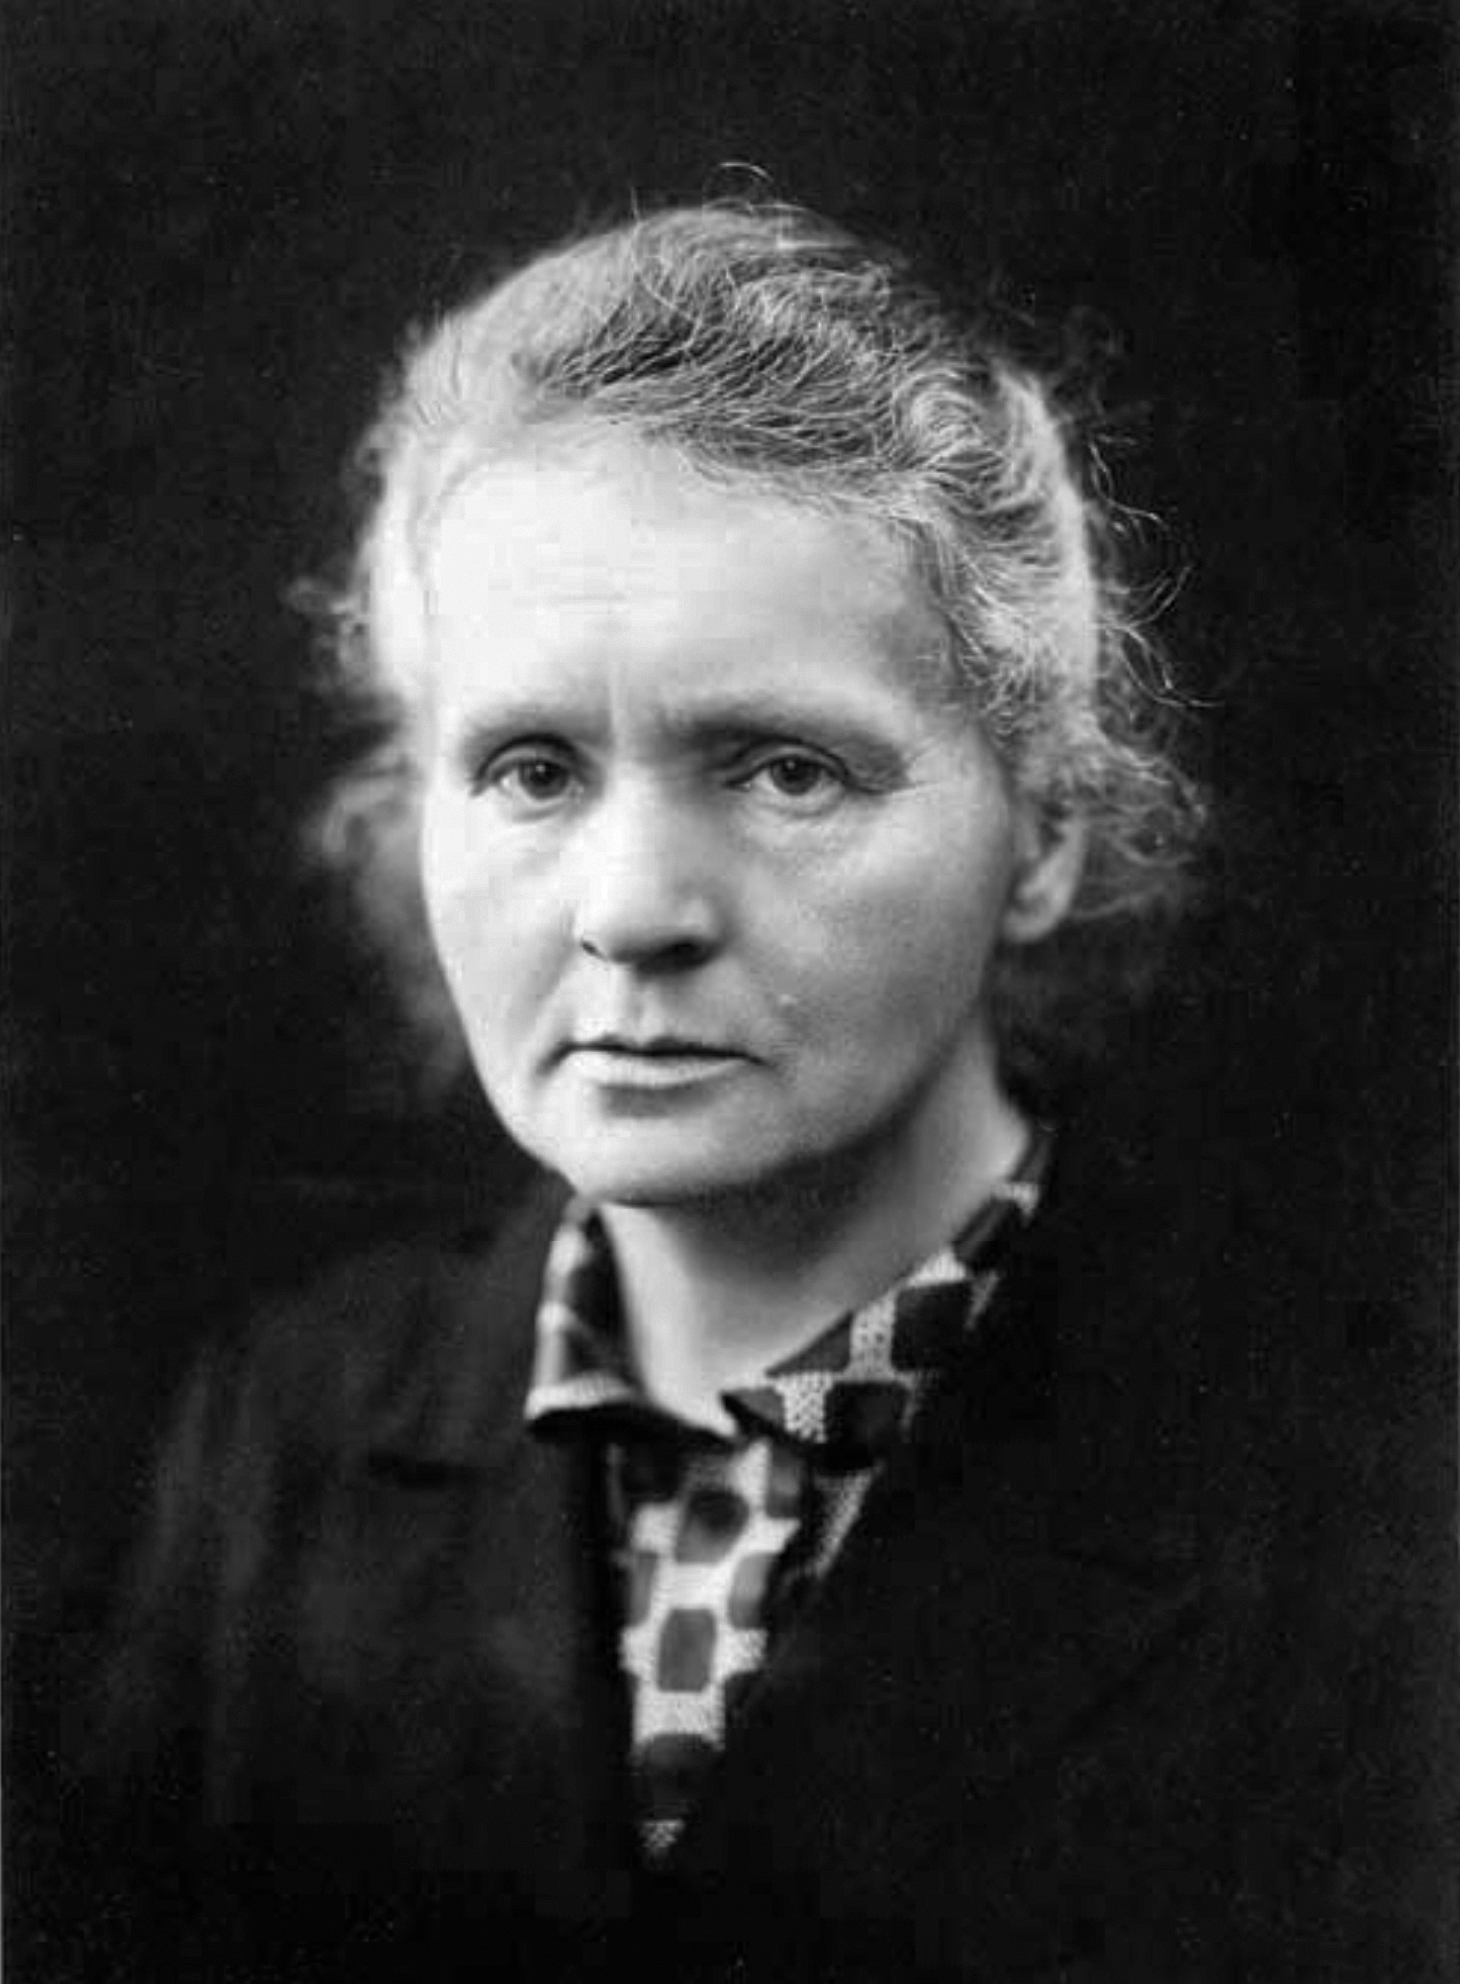
\includegraphics[width=0.34\linewidth]{images/book5/photo-marie-curie.jpg}

{\small Marie Curie (fotografia de Henri Manuel, por volta de 1920, domínio público): duas vezes laureada com o Nobel por abrir o assunto deste capítulo --- o grama de rádio do \cref{exo:b3:nuclear-physics:4} era dela.}
\end{omfigure}

\section{Exercícios}

\begin{exercise}[$\star$]\label{exo:b3:nuclear-physics:1}
Contabilidade. (a) Dê $Z$, $N$, $A$ para $^{12}$C, $^{14}$C,
$^{235}$U, $^{238}$U. (b) Que pares são \omterm{def:b3:nuclear-physics:nuclide}{isótopos}? (c) Por que os
\omterm{def:b3:nuclear-physics:nuclide}{isótopos} compartilham química, mas não estabilidade nuclear? (d) O $^{14}$C
e o $^{14}$N compartilham $A = 14$: como se chamam \omterm{def:b3:nuclear-physics:nuclide}{nuclídeos} assim, e
que decaimento os conecta?
\end{exercise}

\begin{exercise}[$\star$]\label{exo:b3:nuclear-physics:2}
A densidade universal. (a) A partir de $R = r_0A^{1/3}$, mostre que a
densidade nuclear independe de $A$ e avalie-a. (b)
Calcule a massa de uma colher de chá (\qty{5}{mL}) de matéria nuclear.
(c) Que fração do volume de um átomo o núcleo dele preenche (tome
$R_{\text{át}} = \qty{1e-10}{m}$, $A = 60$)? (d) O que a própria lei
$A^{1/3}$ diz sobre o alcance da força forte?
\end{exercise}

\begin{exercise}[$\star$]\label{exo:b3:nuclear-physics:3}
Pesando a cola. Massas nucleares: $m_{\text{p}} =
\qty{1.007276}{u}$, $m_{\text{n}} = \qty{1.008665}{u}$,
$m(^4\text{He}) = \qty{4.001506}{u}$;
$\qty{1}{u}\,c^2 = \qty{931.5}{MeV}$. (a) Calcule o \omterm{thm:b3:relativistic-dynamics:emc2}{defeito de massa}
e a \omterm{prop:b3:nuclear-physics:binding}{energia de ligação} do $^4$He. (b) Dê o $B/A$. (c) Compare o $B$ com
os \qty{13.6}{eV} do \cref{ch:b3:hydrogen-atom}: quantas ordens
de grandeza separam a cola nuclear da atômica? (d) Por que a ligação
excepcional do $^4$He (o pico da figura) faz dele a moeda do
decaimento $\alpha$?
\end{exercise}

\begin{exercise}[$\star$]\label{exo:b3:nuclear-physics:4}
O primeiro curie. Rádio-226: $T_{1/2} = 1600$ anos, massa molar
\qty{226}{g/mol}. Para um grama: (a) conte os núcleos; (b) calcule
o $\lambda$; (c) calcule a atividade e compare com a unidade histórica
$1\,\text{Ci} = \qty{3.7e10}{Bq}$ (definida como exatamente este
grama); (d) quanto do grama sobrevive depois de 4800 anos?
\end{exercise}

\begin{exercise}[$\star\star$]\label{exo:b3:nuclear-physics:5}
A fórmula na prática. Com $a_{\text{V}} = 15.75$,
$a_{\text{S}} = 17.8$, $a_{\text{C}} = 0.711$,
$a_{\text{A}} = 23.7$ (\unit{MeV}) e emparelhamento
$+12/\sqrt A$ para núcleos par--par: (a) calcule os quatro termos
principais de $B$ para o $^{56}$Fe ($Z = 26$). (b) Some (com o
emparelhamento) e compare o $B/A$ com os \qty{8.79}{MeV} medidos. (c)
Que dois termos brigam mais forte, e o que o equilíbrio deles fixa? (d)
Por que o termo de Coulomb, sozinho, tem de crescer \emph{mais rápido}
que $A$?
\end{exercise}

\begin{exercise}[$\star\star$]\label{exo:b3:nuclear-physics:6}
O fundo do vale. (a) Guardando só os termos que dependem de $Z$,
minimize a massa a $A$ fixo e deduza
$Z^* = \dfrac{A/2}{1 + a_{\text{C}}A^{2/3}/4a_{\text{A}}}$. (b)
Avalie para $A = 101$ e compare com o rutênio ($Z = 44$).
(c) Mostre que o limite de $A$ pequeno é $Z^* = A/2$ e interprete com
as duas escadas de Fermi. (d) Um fragmento de fissão tem $A = 95$ e
$Z = 36$: a que distância do vale ele está, e que sequência de
decaimentos vem depois?
\end{exercise}

\begin{exercise}[$\star\star$]\label{exo:b3:nuclear-physics:7}
Radiocarbono. A matéria viva mantém o $^{14}$C
($T_{1/2} = 5730$ anos) reposto a 1 átomo por $10^{12}$
carbonos; a morte interrompe a reposição. (a) Uma amostra de carvão
mostra 30\,\% da atividade viva: que idade tem a fogueira? (b) Um grama
de carbono vivo: calcule a atividade de $^{14}$C dele
($\approx\qty{0.23}{Bq}$ esperados). (c) Por que o método é inútil
além de $\sim\qty{50000}{}$ anos? (d) E por que é inútil para
datar rochas (que relógios assumem)?
\end{exercise}

\begin{exercise}[$\star\star$]\label{exo:b3:nuclear-physics:8}
O penhasco de Gamow. O polônio-212 emite um $\alpha$ de \qty{8.78}{MeV};
a barreira dele chega a $\approx\qty{26}{MeV}$. (a) Mostre que a fuga
clássica é impossível, e a entrada clássica também --- e ainda assim ele
decai em \qty{0.3}{\micro s}. (b) O $\alpha$ do urânio-238 carrega
\qty{4.2}{MeV} e a meia-vida dele é de $4.5\times10^9$ anos:
calcule a razão entre as duas constantes de decaimento. (c) Explique, com
a exponencial do tunelamento, como um fator dois em energia compra
$\sim10^{24}$ em taxa. (d) Por que a mesma física fixa a exigência de
temperatura no núcleo do Sol?
\end{exercise}

\begin{exercise}[$\star\star$]\label{exo:b3:nuclear-physics:9}
Duzentos milhões de elétron-volts. (a) Justifique os
$\qty{200}{MeV}$ por fissão a partir da curva $B/A$. (b) Calcule
a energia de um quilograma de $^{235}$U totalmente fissionado, em
joules e em toneladas equivalentes de petróleo
(\qty{42}{GJ/t}). (c) Uma usina de \qty{1}{GW_e} com 33\,\% de
eficiência: quantos quilogramas de $^{235}$U por ano? (d) Por que
os fragmentos, e não os nêutrons, carregam a maior parte dos
\qty{200}{MeV}, e em que forma isso se converte de imediato?
\end{exercise}

\begin{exercise}[$\star\star\star$]\label{exo:b3:nuclear-physics:10}
Domando o $k$. Num reator, os nêutrons prontos se reproduzem em $\ell
\approx \qty{e-4}{s}$. (a) Com $k = 1.001$ só nos nêutrons prontos,
calcule a multiplicação de potência em um segundo --- e o
veredito sobre controle mecânico. (b) Uma fração $\beta =
0.7\,\%$ dos nêutrons é \emph{atrasada} em $\sim\qty{10}{s}$:
explique por que, para $k - 1 < \beta$, o relógio efetivo da cadeia
passa a ser de segundos. (c) Calcule a mesma multiplicação de um segundo
com o tempo de geração efetivo $\sim\qty{0.1}{s}$. (d) Diga
em uma frase o que os operadores de Chernobyl perderam quando o
reator deles ficou pronto-supercrítico.
\end{exercise}

\begin{exercise}[$\star\star\star$]\label{exo:b3:nuclear-physics:11}
A aritmética do Sol. No conjunto, $4\,^1\text{H} \to {}^4\text{He}$
converte \qty{0.71}{\percent} da massa em energia
(\qty{26.7}{MeV}, neutrinos incluídos). (a) A partir de $L_\odot =
\qty{3.8e26}{W}$, calcule a massa convertida por segundo e o
hidrogênio consumido por segundo. (b) Com $\qty{2e30}{kg}$ de Sol,
e um décimo disso de hidrogênio queimável no núcleo (tome a fração de
hidrogênio $\approx0.75$): estime o tempo de vida. (c) Dois prótons a
\qty{1.5e7}{K}: compare $k_{\text{B}}T$ com a barreira de Coulomb
deles a \qty{1}{fm} e conclua quem faz a travessia
(\cref{exo:b3:nuclear-physics:8}). (d) Por que a fusão, ao contrário da
fissão, não deixa essencialmente cinza radioativa alguma?
\end{exercise}

\begin{exercise}[$\star\star\star$]\label{exo:b3:nuclear-physics:12}
Medicina nuclear. (a) O tecnécio-99m ($T_{1/2} = \qty{6}{h}$,
$\gamma$ de \qty{140}{keV}) é o burro de carga da medicina: calcule o
número de núcleos, e a massa deles, por trás de uma injeção de
\qty{500}{MBq}. (b) Explique por que uma meia-vida de seis \emph{horas} e
um $\gamma$ puro são exatamente o que um diagnóstico quer. (c) PET:
um pósitron do $^{18}$F se aniquila com um elétron ---
use o \cref{ch:b3:relativistic-dynamics} para dar a energia e a
geometria dos dois fótons e, daí, o princípio do detector.
(d) A radioterapia entrega \qty{2}{Gy} (\unit{J/kg}) a um tumor:
compare a energia com um gole de água morna e concilie a
inocuidade dos joules com a letalidade da ionização.
\end{exercise}

\begin{omfigure}
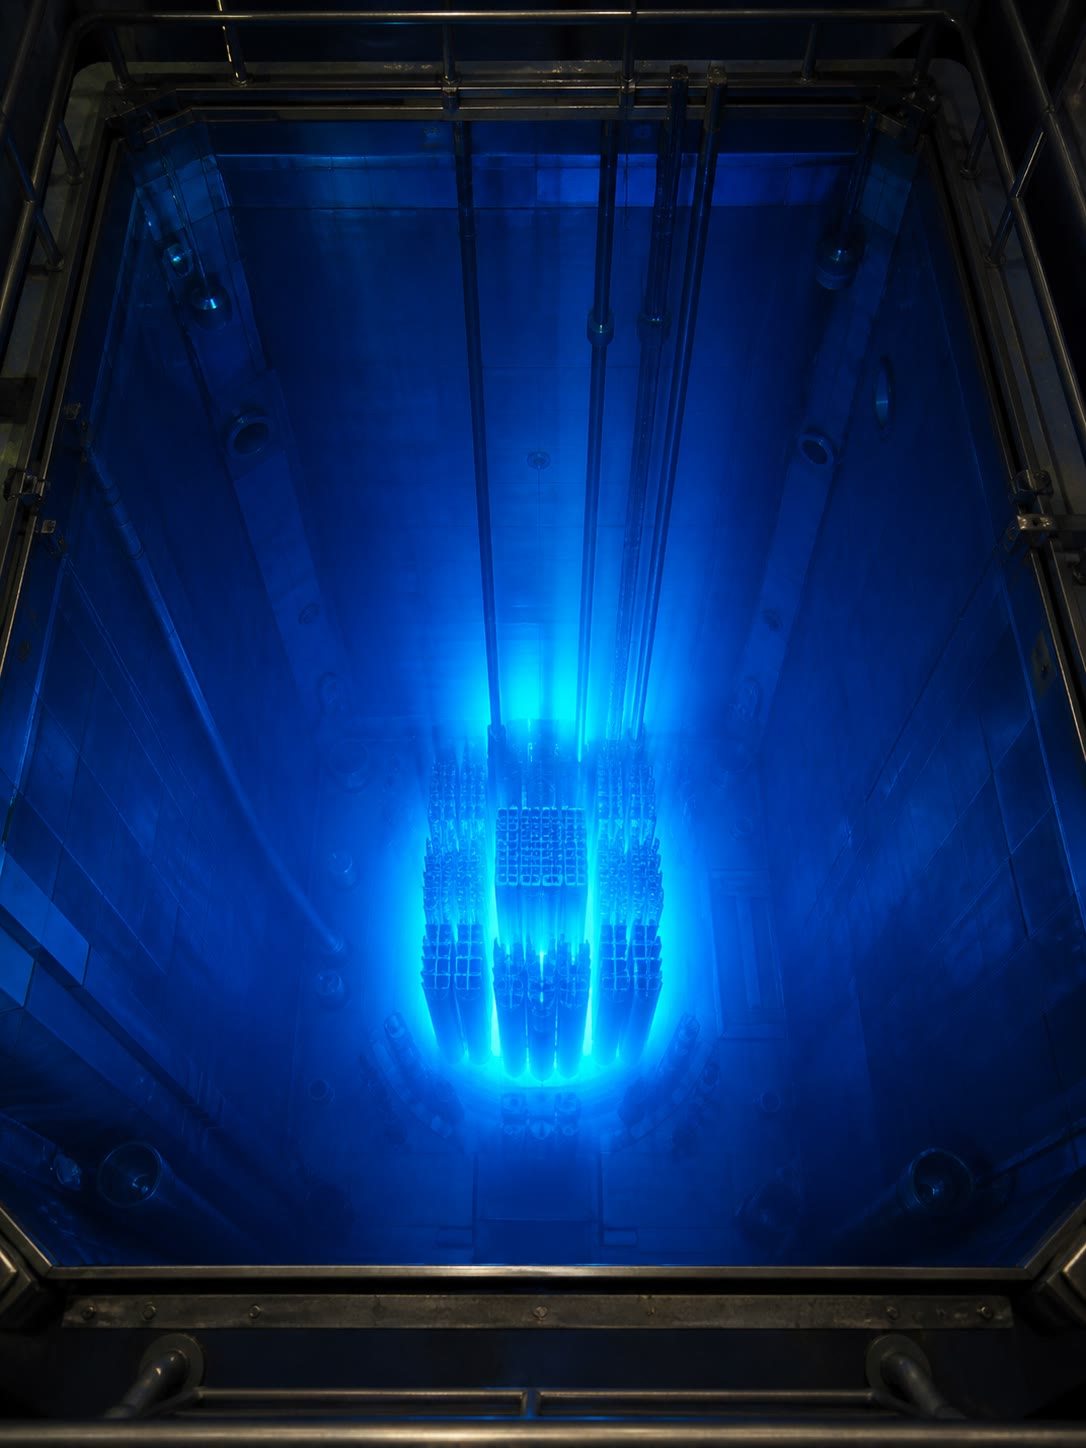
\includegraphics[width=0.45\linewidth]{images/book5/ai/b5-21-cherenkov-pool.jpg}

{\small A piscina de reator do problema de fim de semana: os elétrons $\beta$ dos fragmentos, mais rápidos que a luz na água, envolvem o núcleo no azul de Cherenkov --- a blindagem, visivelmente em ação.}
\end{omfigure}

\section{Problema: dia aberto no reator de pesquisa}

\begin{problem}\label{pb:b3:nuclear-physics:1}
\emph{Dia aberto no reator de pesquisa.} O laboratório nacional
abre a visitantes o reator de pesquisa tipo piscina de \qty{20}{MW}
dele, e você conseguiu na conversa um lugar na sacada: lá embaixo,
por oito metros de água límpida, o núcleo brilha num azul
sobrenatural. O guia --- um físico de reatores prestes a se aposentar
--- concordou em deixar você fazer as contas.

\medskip\noindent\textbf{Parte I --- O livro-caixa da energia.}

\begin{enumerate}
  \item Cada fissão de $^{235}$U libera cerca de \qty{200}{MeV}.
        Converta em joules e calcule as fissões por segundo
        que sustentam \qty{20}{MW}.
  \item Converta em gramas de $^{235}$U consumidos por dia.
  \item Os mesmos \qty{20}{MW} vindos de carvão (\qty{30}{MJ/kg}): quantas
        toneladas por dia? Forme a razão de massas e conecte-a às
        escalas de \unit{MeV} contra \unit{eV} deste capítulo e da
        química.
  \item Os fragmentos nascem com ligação de $\sim\qty{8.5}{MeV}$ por
        núcleon, e o urânio com \qty{7.6}{MeV}: verifique que
        $235\times0.9 \approx \qty{200}{MeV}$ é consistente.
  \item Os fragmentos param a micrômetros do lugar em que nasceram.
        Em que a \qty{200}{MeV} deles se converte, e em que
        escala de tempo isso chega à água de refrigeração?
  \item Por que os fragmentos (por exemplo, $A = 95$, $Z = 36$)
        são inevitavelmente radioativos? Use o \omterm{prop:b3:nuclear-physics:semf}{vale de estabilidade}.
\end{enumerate}

\medskip\noindent\textbf{Parte II --- Mantendo $k = 1$.}

\begin{enumerate}[resume]
  \item Defina o fator de multiplicação $k$ e diga o que
        $k = 0.999$, $1.000$ e $1.001$ significam para a população
        de nêutrons.
  \item A água da piscina modera. Explique em duas frases por que
        frear os nêutrons a velocidades térmicas \emph{ajuda} a fissionar
        o $^{235}$U, e por que o hidrogênio é o melhor moderador
        (lembre as colisões elásticas do volume do primeiro ano).
  \item As barras de controle são de aço com boro. O que o boro faz, e
        como subir ou descer as barras dirige o $k$?
  \item Só com os nêutrons prontos ($\ell = \qty{e-4}{s}$) e
        $k = 1.0005$, calcule o crescimento de potência em um segundo
        e conclua.
  \item Os 0,7\,\% de nêutrons atrasados esticam o tempo de geração
        efetivo até $\sim\qty{0.1}{s}$: recalcule e
        enuncie a regra de projeto que mantém $k - 1$ com folga abaixo
        da fração atrasada.
  \item A água também é o refrigerante. Explique o traço de segurança
        intrínseca: o que acontece com a moderação --- e portanto
        com o $k$ --- se a água ferver e sumir?
  \item Por que o reator ainda precisa de refrigeração de emergência
        depois do desligamento? (Nomeie a fonte de calor que as barras
        de controle não conseguem tocar.)
\end{enumerate}

\medskip\noindent\textbf{Parte III --- A luz azul.}

\begin{enumerate}[resume]
  \item O brilho é radiação Cherenkov: a velocidade da luz na água
        é $c/n$, com $n = 1.33$. O que uma partícula carregada tem
        de fazer para emiti-la?
  \item Calcule a velocidade limiar e, com o
        \cref{ch:b3:relativistic-dynamics}, a energia cinética
        limiar de um elétron.
  \item Que partículas do reator se qualificam? Trace a cadeia do
        fragmento de fissão ao elétron $\beta$ rápido na água.
  \item A intensidade do espectro cresce rumo aos comprimentos de onda
        curtos: por que a piscina brilha em azul, e não em vermelho?
  \item O guia diz: ``o brilho \emph{é} a blindagem
        funcionando''. Explique --- o que oito metros de água fazem
        com a radiação do núcleo, e por que, grosso modo, a sacada é segura?
  \item Depois do desligamento, o azul se apaga ao longo de minutos, mas
        não some por dias. Conecte com a questão 6 da Parte I.
\end{enumerate}

\medskip\noindent\textbf{Parte IV --- Para que serve o reator.}

\begin{enumerate}[resume]
  \item O trabalho do dia a dia deste reator é fazer molibdênio-99
        ($T_{1/2} = \qty{66}{h}$), pai do tecnécio-99m da
        medicina. Por que os hospitais do mundo têm de ser
        reabastecidos toda semana, e por que armazém algum consegue estocá-lo?
  \item Um carregamento de \qty{100}{GBq} de Mo-99 parte na segunda; o
        hospital elui o Tc-99m na sexta (96 horas depois). Que
        atividade do pai resta?
  \item Os feixes de nêutrons do núcleo também alimentam os
        instrumentos de difração do \cref{ch:b3:crystalline-solids}: por que
        os nêutrons de reator, uma vez termalizados, nascem com o
        comprimento de onda certo?
  \item O problema de despedida do guia: um elemento combustível passa
        cinco anos na piscina antes de ser embarcado. Usando a
        mistura de meias-vidas dos fragmentos, explique a lógica --- o que
        cinco anos de piscina compraram?
  \item Estime o calor de decaimento uma hora depois do desligamento
        ($\approx1\,\%$ de \qty{20}{MW}) e compare-o com o
        aquecedor elétrico de uma casa: a refrigeração passiva da piscina
        é plausível?
  \item Feche o livro-caixa em quatro linhas: o $B/A$ paga
        \qty{200}{MeV} por partição; os nêutrons atrasados emprestam os
        segundos que tornam o $k$ dirigível; a água modera,
        resfria, blinda e brilha; e o produto de verdade do dia
        sai em frascos médicos, não em megawatts.
\end{enumerate}
\end{problem}
